


% \section{Handling Sparse Learning Signal}

% \label{sec:analysissection}

% To start our investigation, we seek to understand how learning works for LCLMs on high-\cname tasks. In particular, we will investigate gradient sparsity and potential solutions on some complex tasks.

% % \prasannnote{Amanda gave a nice suggestion to adjust framing mask-mixing as extra support since it removes alternative explanations for complexity gap, so I adjusted writing to reflect that}




% % \prasannnote{RYAN: maybe unify visualization color scheme?}

% \subsection{Analysis: Sparse Gradients and Natural CoTs}

% \begin{figure*}[t]
% \centering
% 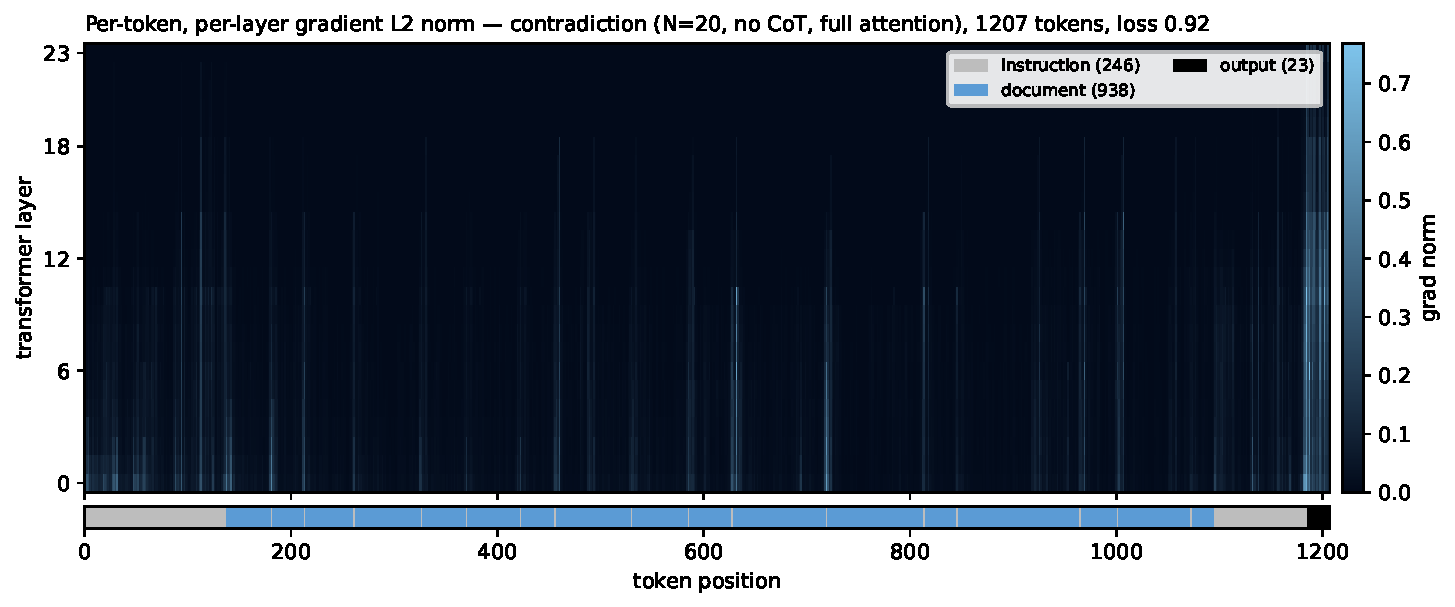
\includegraphics[width=.95\linewidth]{figures/section6_gradnorm.pdf}
% % \vspace{-.2em}
% \caption{\emph{Layer/token gradient L2 norm for one contradiction example} (Qwen-3.5-0.8B-Base, fresh LoRA, full causal attention, $N{=}20$, no CoT, 1207 tokens, loss 0.92). Rows are transformer layers (early at the bottom), columns token positions, lighter color indicates higher norm. Strip below marks different kinds of tokens. Signal is heavily concentrated: 1\% of cells carry 17.6\% of gradient mass; top 5\% of cells carry 46.5\%. \textbf{Most representations receive essentially zero update.}}
% \label{fig:gradnorms}
% % \vspace{-.2em}
% \end{figure*}


% % \prasannnote{I think we should avoid making big claims here, but these analyses probably add some coolness factor which I think makes them worth including}

% To better understand how LCLMs learn corpus  reasoning tasks, we start with a simple analysis: \emph{what does a single LCLM gradient step look like}?  We show a visualization of language model gradient norms during training (albeit with a small 0.8B model at an initial training step) in Figure~\ref{fig:gradnorms}, where the loss is with respect to just answer tokens. As we can see in the figure, while learning signal is dense over the query and answer, \textbf{the learning signal over document representations is incredibly sparse}, and most token representations aren't being meaningfully updated at most layers.


% Without updating correct parts of context, training can slow down or fail. We hypothesize LCLM learning to be dependent on what a model may initially attend to / update. This can play a role in differing behavior between different \cname tasks. For instance, in HPQA there's \textbf{(a)} heavy word overlap between query and context, and so we might expect learning to be much more data efficient and easy. Conversely, for the outlier setting, where there's \textbf{(b)} minimal signal per question about which part of contexts to examine, learning may, independent of architecture, be quite challenging.  

% \begin{wraptable}{r}{0.48\textwidth}
% \centering
% \small
% \setlength{\tabcolsep}{4pt}
% \begin{tabular}{lc}
% \toprule
% CoT target & F1 \\
% \midrule
% Faithful (majority/minority labels) & \textbf{0.734} \\
% Repeat gold outlier IDs & 0.594 \\
% Mislabeled (wrong majority/minority) & 0.097 \\
% Dummy (content-less phrase) & 0.097 \\
% Random words from context & 0.007 \\
% Dummy CoT + smoothing ($\alpha{=}0.8$) & 0.106 \\
% \midrule
% Random baseline (3 of 30) & 0.100 \\
% \bottomrule
% \end{tabular}
% \caption{\emph{Outlier-task CoT ablation} (Qwen-3.5-0.8B-Base, $N{=}30$, 500 eval examples). \textbf{Faithful CoTs help the most}; mislabeled, content-free, and random-word CoTs all match chance, as does direct attention smoothing.}
% \label{tab:cot-ablation}
% \end{wraptable}

% We find an initial intuitive fix to often help in this setting: natural chains-of-thought. If answer tokens contain pointers to the right parts of context (e.g document ids, natural language), this may mitigate problem (b). We tune CoT schemes across all our settings (including HPQA, a simpler setting), and find that even simple approaches can improve both chunked and standard performance (e.g. roughly 0.1 recall on HPQA, or 0.6-0.7 recall on the outlier task where even standard attention learning can depend on CoTs).  



% \textbf{Result:} To shed more insight, we use an Amazon Reviews version of the outlier task (see Appendix~\ref{app:amazon-reviews}), where we note inclusion of CoTs to be particularly important. We in Table~\ref{tab:cot-ablation} show various different kinds of CoTs, and their effect on learning (a ``faithful'' CoT stating majority / outlier category name before answering, a mislabelled CoT)... We also include an attention smoothing baseline where we have the attention of query / answer tokens follow a curriculum where at the beginning of training heavily smooths attention over document tokens. \textbf{Only the correct CoT and answer repetition help}, suggesting the importance of boosting gradient signal on the relevant parts of contexts over less relevant parts. 



% \begin{table}[t]
% \centering
% \small
% \setlength{\tabcolsep}{5pt}
% \begin{tabular}{llccccc}
% \toprule
% \textbf{Task} & \textbf{Model} & $\bm{N}$ & \textbf{Metric} & \textbf{Pure chunked} & \textbf{+ Mask mixing} & $\bm{\Delta}$ \\
% \midrule
% Contradiction          & Qwen-2.5-3B   & 20  & F1   & 0.018          & \textbf{0.987} & +0.97 \\
% Contradiction          & Qwen-3.5-2B   & 20  & F1   & 0.598          & \textbf{0.999} & +0.40 \\
% Contradiction          & Qwen-3.5-2B   & 100 & F1   & 0.001          & \textbf{0.737} & +0.74 \\
% Grouping (OpenAlex)    & Qwen-3.5-4B   & 50  & pwF1 & 0.389          & \textbf{0.462} & +0.07 \\
% Outlier (wiki, scale-$k$) & Qwen-3.5-4B & 100 & F1   & \textbf{0.518} & 0.503          & $-$0.02 \\
% Reorder (Gutenberg)    & Qwen-3.5-9B   & 20  & $\tau$ & 0.070          & \textbf{0.193}          & +0.12 \\
% \bottomrule
% \vspace{.2em}

% \end{tabular}



% \caption{\emph{Mask mixing vs.\ pure chunked across tasks and scales.} We report mask mixing results for a variety of model and task conditions. Mix probability $p{=}0.10$ \textbf{Mask mixing leads to consistent and large gains for chunked inference on many tasks}}
% \label{tab:mask-mix-suite}
% \end{table}

% \subsection{Mask Mixing}

% Chunked attention with sparse masks suffers may suffer even more from gradient sparsity. We propose an effective new approach---mask mixing---that bridges learning signal gaps. The approach is simple: during chunked attention training, which involves training an LCLM with a chunked mask (see Figure~\ref{fig:masks}), we mix in a random $p$ percentage of full attention mask training batches into training, and \emph{then use chunked attention for evaluation}. $p=0$ is equivalent to chunked attention, and $p=1$ is just full attention training.

% \textbf{Results} We report mask mixing results in Table~\ref{tab:mask-mix-suite} on a few examplar settings. While we find this doesn't work for all tasks, and is most effective with Qwen-3.5 models, \textbf{for several settings, mask mixing improves performance over pure chunked.} We believe this style of generalization / distillation could be an effective lever to getting cheaper approaches to scale further on high \cname tasks. This is potentially related to other results where attention representations are distilled (e.g. in vision \citep{Zagoruyko2016PayingMA}). We hypothesize that chunked attention may be out-of-distribution or unable to update the right representations, and so occasionally updating with standard attention can warm-start the representations.



% \subsection{Is Natural Guidance Actually Important?}

% While our results provide some initial support for the hypothesis of this section -- that greater natural language pointers to relevant parts of context otherwise missed with shallow heuristics aid learning -- there are still alternative explanations to our findings. We here test a variety of these hypotheses to validate our initial hypothesis.

% \paragraph{Does Any CoT Work?} \prasannnote{more details needed on CoT construction somewhere} One question that may arise is whether the specific CoTs we use matter, or if any roughly plausible content is fine. To test this, we train Qwen-3.5-0.8B-Base on the outlier task ($N{=}30$ Amazon reviews, 5k train examples) with the same data and hyperparameters but five different CoT targets: a faithful CoT that names the majority and minority attribute (e.g.\ ``Most reviews are 4-star ratings and the outliers are 5-star reviews.''), a \emph{repeat-IDs} CoT that just emits the gold outlier IDs before the answer line, a \emph{mislabeled} CoT with the same template as faithful but a randomly-permuted (wrong) majority/minority pair, a \emph{dummy} content-less phrase (``I'll first look for the majority \{rating, category\} before outputting the final IDs.''), and a \emph{random words} CoT consisting of 50 content words sampled from the input documents. Results in Table~\ref{tab:cot-ablation} make the picture clear: only the semantically faithful CoT comes close to closing the gap, while a target that merely surfaces the answer IDs as scaffolding gives a meaningful but smaller bump. Mislabeled, dummy, and random-word CoTs collapse to roughly the random-baseline F1 of 0.10, and random words additionally derails the model's ability to emit a parseable answer.


% That said, CoTs are not a cure-all. They aren't able to help overcome scaling limits of computation which we examined in Section~TODO, and sometimes need to be quite long to work well, in particular for the contradiction setting which we find requires longer CoTs that scale with corpus size, with shorter versions not being quite effective.


% \paragraph{Can This Be Fixed with Smoothing?} Another question is whether this is simply an issue with bad initialization, and where perhaps simply smoothing attention could help. To test this, we experiment with smoothing attention scores for query / answer tokens across context to encourage models to, early in training, have an equal chance of attending to and thus updating representations across the corpus. We find that smoothing, with a few different curriculum, does not really help performance. 


% \prasann{TODO need to check if this is maybe not an issue for bigger models (with more high-level / versatile representations)}

% \prasann{below are residual notes, sort of covered but leaving for a better pass later}

% - Start with a figure illustrating how sparse learning can break when a task isn’t a simple O(N) / show visualization with gradient norm maps. Can potentially connect to sparse attention, etc.

% - Figure: Demonstrate how attention can be sparse in bad ways, how CoT can help

% - CoTs: Connect to Agentic RAG / RLMs / related work in that space. 

% - Discuss gains from including natural language guidance (CoTs) across domains

% - Contrast this with CoT in shorter versions of the task, show that the gain (or naturalness) is particularly beneficial in longer context settings

% - Table: Show CoT gains on various settings for chunked / not

% - Table: Show CoT for different kinds of CoT to validate that correct / natural is most important (outlier task)

% - CoTs aren’t a cure-all -> Discuss how they can partially but not fully rescue chunked attention

% \prasannnote{Some positive CoT signal for contradiction task, but only when scaled to be almost as long as corpus size, which defeats the point? Can talk about it / bulk experiments if that seems interesting.}

% \prasannnote{I realize that we're leaving a lot of open questions here. Should probably clean up more / investigate either post-deadline or earlier.}

% \amandanote{I like this explanation a lot more than the framing at the start of the section about narrowing the gap. I wonder if a better framing for mask mixing is more like: (0) LCLM have very sparse gradient, which might be part of why it's hard to learn in sparse settings; (0.5) natural CoT helps with this; (1) is this the only reason chunked settings underperform? (2) we come up with a patch for this problem, mask mixing, [...] (3) this helps strengthen the chunked attention baselines! (4) but the fundamental gap from CTC remains :( (5) so analysis of learning dynamics can improve from existing approaches, but we still leave this open problem for the future. This would be more of a ``mask mixing is evidence that strengthens our claim that CTC is the underlying factor limiting performance (because we see the CTC gap after we use mask mixing to remove a different, adjacent limiting factor)'' framing.} \prasannnote{Ah that's a good idea!}

% Mask-mixing ratio ablation moved to Appendix~\ref{app:mask-mix-ablation}.
